\documentclass[]{article}

\usepackage{geometry}
\geometry{
	top=8mm,
	left=15mm,
	right=15mm
}

\usepackage{graphicx}
\graphicspath{.}

\usepackage{hyperref}
\hypersetup{
	colorlinks=true,
	urlcolor=blue
}

%opening
\title{Visual Analytics project proposal: European parties explorer}
\author{Stefano Bonetti, 1764624}
\date{}

\begin{document}
	
\maketitle
	
\section{General idea}
What follows is an idea for a visual analytics system suited for tasks like exploring how European political parties have evolved in the last years, how their views over the most important topics have changed, comparing parties in one or many countries, viewing how polarized nations or political factions are on certain topics, and possibly discovering further similar insights. The political parties will be represented in different charts and filtered according to the year, the country they come from, and their political factions (left, right, etc.), while obviously allowing brushing too.

\section{The dataset and the Chapel Hill Expert Surveys}
An interesting dataset I found was based on the \href{https://www.chesdata.eu/}{Chapel Hill Expert Surveys} (CHES), a set of surveys conducted in 1999, 2002, 2006, 2010, 2014, 2019 and 2024 which were distributed to many political experts so that they could evaluate the most important parties in many European nations. The site contains two \href{https://www.chesdata.eu/ches-europe}{datasets}, one for all surveys from 1999 to 2019 and one for the latest survey in 2024, so I will probably need to do a little work to join them together in a single dataset.\\
Each row in the dataset represents a major European party and how it was evaluated by the experts in one of the given years; each column contains either information about the party (e.g. country, ID, name, votes) or, most importantly, a number assigned by the experts representing the party's opinion on a certain topic (for instance, a low score on the attribute EU\_POSITION means that party is eurosceptic, a high score that it is europeist).\\
The various parties were evaluated on a lot of topics, so the full dataset has an AS index that is actually way higher than requested. For this reason, I will only use a subset of the attributes (the most important topics), also because some of them are very redundant or were assigned by the expert only during one or two years (so they wouldn't be very useful). I will likely use the following attributes: year, country, party ID, party name, votes received, political faction, opinion on EU, ideological stance (left/right), ideological stance on the economy, deregulation of markets, redistribution of wealth, civil liberties, LGBT rights, religious principles, immigration policy, multiculturalism, urban vs. rural interests, environment, regionalism, ethnic minorities, Russian interference, anti-Islam rhetoric; this gives an overall AS index of almost 32500. I may consider adding or exchanging attributes if needed.

\section{Draft}
\begin{itemize}
	\item The application will allow the user to filter political parties according to the year in which they were evaluated, their country of origin, and their political faction; all visualizations will be updated appropriately.
	\item A dimensionality reduction technique will be used for a scatter plot in which every party will be represented as a bubble whose size depends on the votes received, and the bubbles will be colored based on the country of origin or the political family. As dimensionality reduction I will try to use MDS, since intuitively we could define a dissimilarity matrix based on the parties' scores over the many topics.
	\item A line chart will show the evolution over time of the parties with respect to a topic selected by the user (for instance, we could see a party becoming less eurosceptic); this will be the only chart not affected by the selected year, since it will have to show parties over time.
	\item The parallel coordinates plot will represent political parties as lines, visualizing in one single chart all topics on which they were evaluated and their scores.
	\item Finally, there will be some box plots, quickly showing how the filtered parties are distributed on the hottest topics.
\end{itemize}
Of course, brushing will be available on both the scatter plot and the parallel coordinates, and the changes will be reflected on all other visualizations. I will also try to find a way to explain how the scores work on the various topics, to make them clear to the user (e.g. a low score on LGBT rights means "against").
\begin{figure}[h]
	\centering
	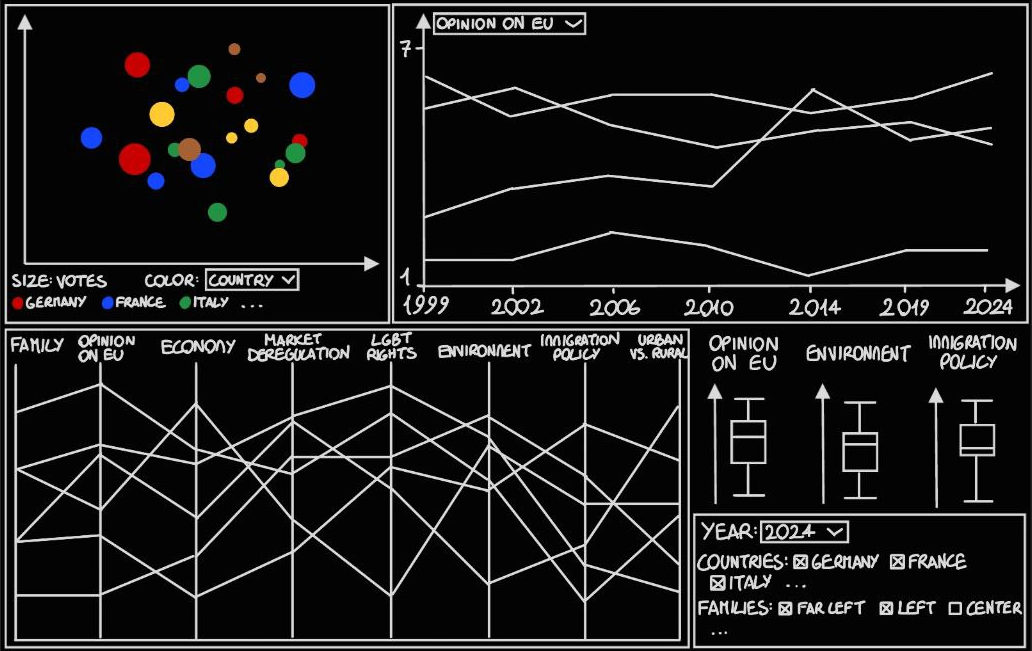
\includegraphics[scale=0.4]{draft.png}
\end{figure}
	
\section{Intended users}
Some possible users can be researchers, experts or students in political science whose aims could be, as mentioned in the beginning, analyzing ideological evolutions of political parties or nations over time, comparing similar parties from different countries, observing how polarized a political faction is on a specific topic, finding outlier parties, etc. The application could be useful to journalists and the like too, since they may want to write articles based on historical data, or tell how some parties have evolved during the years.\\
Another possible but maybe less likely user is a simple citizen who is about to vote for the national or European elections and wants to better "study" the parties they can vote for, or check how "coherent" a given party has been regarding specific topics during the years.

\end{document}
